\documentclass[aspectratio=169,10pt,t]{beamer}
% \usetheme[
% %%% options passed to the outer theme
% %    progressstyle=fixedCircCnt,   %either fixedCircCnt, movCircCnt, or corner
% %    rotationcw,          % change the rotation direction from counter-clockwise to clockwise
% %    shownavsym          % show the navigation symbols
%   ]{SDUsimple}
\usepackage{SDUtheme/beamerthemeSDUsimple}
% If you want to change the colors of the various elements in the theme, edit and uncomment the following lines
% Change the bar and sidebar colors:
%\setbeamercolor{SDUsimple}{fg=red!20,bg=red}
%\setbeamercolor{sidebar}{bg=red!20}
% Change the color of the structural elements:
%\setbeamercolor{structure}{fg=red}
% Change the frame title text color:
%\setbeamercolor{frametitle}{fg=blue}
% Change the normal text color background:
%\setbeamercolor{normal text}{fg=black,bg=gray!10}
% ... and you can of course change a lot more - see the beamer user manual.
\usepackage{color}
\usepackage{float}
\usepackage{dsfont}                         % Enables double stroke fonts
\usepackage{bm}
\usepackage[utf8]{inputenc}
\usepackage[english]{babel}
\usepackage[T1]{fontenc}
\usepackage{listings}
% Or whatever. Note that the encoding and the font should match. If T1
% does not look nice, try deleting the line with the fontenc.
\usepackage{helvet}
\usefonttheme{professionalfonts}

\newtheorem{algorithm}{Algorithm}
%\newtheorem{problem}{Problem}
\newtheorem{proposition}{Proposition}
% colored hyperlinks
\newcommand{\chref}[2]{%
	\href{#1}{{\usebeamercolor[bg]{SDUsimple}#2}}%
}

\title{Regression and the General Linear Model}
\subtitle{Multivariate Statistic}
%\date{\today}
\date{ }

\author{
	Made by: \\
	\textbf{Lasse Gøransson, Marc Evald, Anne-Charlotte Poulsen \& Aske Møller}
}

% - Give the names in the same order as they appear in the paper.
% - Use the \inst{?} command only if the authors have different
%   affiliation. See the beamer manual for an example

\institute[
%  {\includegraphics[scale=0.2]{SDU_segl}}\\ %insert a company, department or university logo
SDU Robotics\\
The Maersk Mc-Kinney Moller Institute\\
University of Southern Denmark
] % optional - is placed in the bottom of the sidebar on every slide
{% is placed on the bottom of the title page
	SDU Robotics\\
	The Maersk Mc-Kinney Moller Institute\\
	University of Southern Denmark

	%there must be an empty line above this line - otherwise some unwanted space is added between the university and the country (I do not know why;( )
}

% specify a logo on the titlepage (you can specify additional logos an include them in
% institute command below
\pgfdeclareimage[height=0.5cm]{titlepagelogo}{SDUgraphics/SDU_logo_new} % placed on the title page
%\pgfdeclareimage[height=1.5cm]{titlepagelogo2}{SDUgraphics/SDU_logo_new} % placed on the title page
\titlegraphic{% is placed on the bottom of the title page
	\pgfuseimage{titlepagelogo}
	%  \hspace{1cm}\pgfuseimage{titlepagelogo2}
}

\begin{document}
% the titlepage
{\SDUwavesbg%
	\begin{frame}[plain,noframenumbering] % the plain option removes the header from the title page
		\titlepage
\end{frame}}
%%%%%%%%%%%%%%%%

\begin{frame}[t]
	\frametitle{Agenda}

	\begin{itemize}
		\item Motivation
		\item UMLR
			\begin{itemize}
				\item Model
				\item Estimation
				\item Model Check
				\item Inference on $\beta$
				\item Model reduction
			\end{itemize}
		\item MMLR
	\end{itemize}
	
\end{frame}

\begin{frame}[t]
	\frametitle{Motivation}

    \begin{figure}[H]
    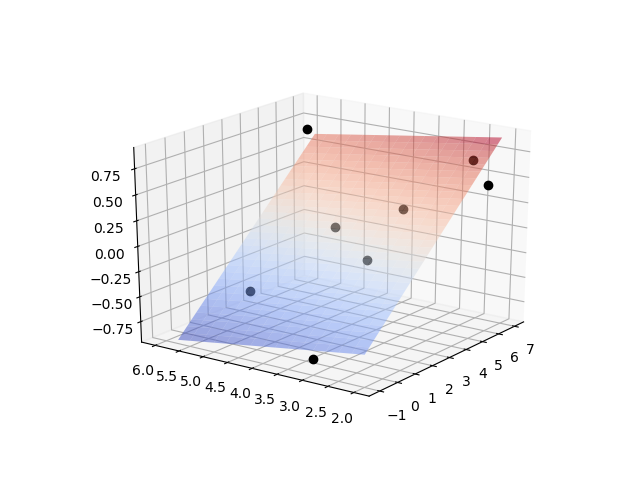
\includegraphics[scale=0.6]{images/regress.png}
    \end{figure}

\end{frame}

\begin{frame}[t]
	\frametitle{Assumptions}

	\begin{itemize}
		\item 
			\[
			Y = z \beta + \epsilon
			\] 
		\item 
			\[
				E  \left[ \epsilon  \right] = 0
			\] 
		\item 
			\[
				V  \left[ \epsilon  \right] = \sigma^{2}
			\] 
	\end{itemize}

	\[
		\begin{bmatrix}
			Y_1\\
			\vdots\\
			Y_{n}
		\end{bmatrix}
		=
		\begin{bmatrix}
			1 & z_{11} & z_{12} & \cdots & z_{1r}\\
			1 & z_{21} & z_{22} &  & \vdots\\
			\vdots & & & \ddots & \\
			1 & z_{n1} &   \cdots && z_{nr}\\
		\end{bmatrix}
		\begin{bmatrix}
			\beta_0\\
			\beta_1\\
			\vdots\\
			\beta_r
		\end{bmatrix}
		+
		\begin{bmatrix}
			\epsilon_1\\
			\epsilon_2\\
			\vdots\\
			\epsilon_n
		\end{bmatrix}
	\] 

\end{frame}

\begin{frame}[t]
	\frametitle{Estimation of Coefficients}
	\[
		\begin{aligned}
			\left( z^{T} z  \right)& ^{-1} &z^{T} Y &= \hat{\beta}_{LS}\\
			\left( z^{T} z  \right)& ^{+} &z^{T} Y &= \hat{\beta}_{LS}
		\end{aligned}
	\] 
\end{frame}

\begin{frame}[t]
	\frametitle{Model check}
	
	\[
		\begin{aligned}
			\sum^{n}_{j=1} 
			\left( Y_j -\bar{Y}   \right)
			\left( Y_j -\bar{Y}    \right) ^{T}
			&=
			\sum^{n}_{j=1} 
			\left( Y_j -\hat{Y}_{j}  \right)
			\left( Y_j -\hat{Y}_{j}  \right)^{T}
			&+
			&\sum^{n}_{j=1}& 
			\left( \hat{Y}_{j} - \bar{Y}  \right) 
			\left( \hat{Y}_{j} - \bar{Y}  \right) ^{T} \\
			\pause
			SST &= SSE &+ &SSR
		\end{aligned}
	\] 

	\[
	 \begin{aligned}
		 R^{2} &= \frac{SSR}{SST} \\
		 \pause
		 R^{2}_{adj} & = 1 - \frac{ \left( n-1 \right) SSE}{ \left( n-r-1 \right) SST} 
	 \end{aligned}
	\] 
\end{frame}

\begin{frame}[t]
	\frametitle{Inference on $\beta$}

	New assumption.


	\[
		\left( \hat{\beta} - \beta^{*}\right) ^{T}
		\left( \frac{Z^{T}Z}{ \left( r+1 \right) \sigma^{2}}   \right) 
		\left( \hat{\beta}  -\beta^{*}\right) 
		\sim
		F_{r+1,n- \left( r+1 \right) }
	\] 

	\pause
	\begin{itemize}
		\item Hypothesis Test
		\item Confidence Region
	\end{itemize}

	
\end{frame}




\begin{frame}[t]
	\frametitle{Model reduction}

	\[
	\beta
	=
	\begin{bmatrix}
		\beta_{ \left( 1 \right) }\\
		\beta_{ \left( 2 \right) }
	\end{bmatrix}
	\begin{matrix}
		\left( q+1 \right) \\
		\left( r-q \right) 
	\end{matrix}
	\] 
	\pause
	\[
		\begin{gathered}
		ESS = \Delta SSR =
		SSR_{\beta} 
		-
		SSR_{\beta_{ \left( 1 \right) }} \\
		\frac{1}{ \sigma^{2}} 
		\cdot
		\frac{ESS}{r-q} 
		\sim
		F_{r-q,n- \left( r+1 \right) }
		\end{gathered}
	\]

\end{frame}

\begin{frame}[t]
	\frametitle{MMLR}
	\framesubtitle{Model}

	 \[
		 \begin{bmatrix}
			 y_{11} & \cdots & y_{1p}\\
\vdots& &\vdots\\
			 y_{n1} & \cdots & y_{np}
		 \end{bmatrix}
		 = 
		\begin{bmatrix}
			1 & z_{11} & z_{12} & \cdots & z_{1r}\\
			1 & z_{21} & z_{22} &  & \vdots\\
			\vdots & & & \ddots & \\
			1 & z_{n1} &   \cdots && z_{nr}\\
		\end{bmatrix}
		\begin{bmatrix}
			\beta_{01} & \cdots & \beta_{0p}\\
			\vdots && \vdots\\
			\beta_{0r} & \cdots & \beta_{rp}
		\end{bmatrix}
		+
		\begin{bmatrix}
			\epsilon_{11} & \cdots & \epsilon_{1p}\\
			\vdots & & \vdots \\
			\epsilon_{n1} & \cdots & \epsilon_{np}
		\end{bmatrix}
	\] 

	
\end{frame}

\begin{frame}[t]
	\frametitle{MMLR}
	\framesubtitle{Model reduction}

	\[
	\Lambda =
	\frac{\max L \left( \beta_{ \left( 1 \right) }   , \Sigma \right) }
	{\max L  \left( \beta ,\Sigma  \right) } 
	=
	 \left( 
		 \frac{ | \hat{\Sigma} |}{| \hat{\Sigma}_{ \left( 1 \right) }|} 
		  \right) 
		 ^{ \frac{n}{2} }
	\] 

	\pause

	\[
	\hat{\Sigma} = \hat{\epsilon}^{T} \hat{\epsilon}
	\] 

	\pause

	\[
		-2 \log  \left( \Lambda  \right) 
		=
		-
		\only<4>{ \left( }
		n
		\only<4>{
		- \left( r+1 \right) 
		- \frac{p-r+q+1}{2} 
	\right) }
		\log  \left( 
			\frac{| \hat{\Sigma}|}{|\hat{\Sigma}_{ \left( 1 \right) }|} 
			 \right) 
			 \underset{approx}{\sim}
			 \chi^{2}_{ \left( r-q \right) p}
	\] 


\end{frame}

\end{document}
